\documentclass{article}
\usepackage{enumerate}
\usepackage[margin=0.8in]{geometry}
\usepackage{hyperref}
\usepackage{graphicx}
\usepackage{wrapfig}
\usepackage[multiple]{footmisc}
\graphicspath{ {userStudyImgs/} }
\begin{document}

\title{PurlPal User Study}
\author{Laura Eckman}
\maketitle

\section{Study Design}

\subsection{Quantitative Evaluation}

Two patterns were involved in this experiment (Figure \ref{patterns}).
Pattern A was 4 rows of 10 stitches each where the 3rd and 7th stitches formed a stockinette column.
Pattern B was 4 rows of 10 stitches each where the first two and last two stitches formed a garter border.

\begin{wrapfigure}{r}{0.4\textwidth} %this figure will be at the right
    \centering
    \includegraphics[width=.39\textwidth]{patterns}
    \caption{Pattern A (left) and Pattern B (right), as presented to participants.} \label{patterns}
\end{wrapfigure}


Participants recruited from a knitting group on campus began knitting in ``Continental'' style with pattern A or pattern B with equal probability to counterbalance any effects of an unintentionally ``harder'' pattern.
For both conditions, the number of changes in visual attention from looking at the screen to looking at their knitting were noted.
The number of times the participant made a mistake and went back to correct it was also noted.
Furthermore, the participants were timed from their first completed stitch until they finished the section or stopped knitting.

Difficulties participants had in utilizing certain functionality in PurlPal and instances when undesired behavior was accidentally produced were also recorded.

\medskip

\textbf{Condition 1: Knitting with Electronic Pattern}

Study participants were given a charted pattern displayed exactly the same way as in PurlPal, but without any row/stitch highlighting or navigational ability. See \ref{nonresponsive} for an example.

\medskip

\textbf{Condition 2: Knitting with PurlPal}

Study participants were read a scripted introduction (\ref{script}) to the features of PurlPal.
Then, study participants observed the researcher knit a single row to demonstrate the necessary proximity to the sensor.
Participants were guided through the calibration process, then began knitting with PurlPal (\ref{responsive}).

\medskip

After knitting, participants filled out a qualitative evaluation of PurlPal (\ref{questionnaire}).

\subsection{Qualitative Study}

I was unable to find more than 2 participants to participate in my study after the pilot tests, so I additionally recruited 40 knitters from an online group to evaluate the interface based on the demo videos recorded for class.\footnote{https://www.youtube.com/watch?v=mjchJaeXPV8}\footnote{https://www.youtube.com/watch?v=uapxhQTu23c}
Even though these participants were unable to actually use the interface to provided empirical feedback, having many more knitters fill out the information survey (\ref{participant-info}) and qualitative evaluation (\ref{questionnaire}) allowed me to get enough data on these questions to form a good picture of preferences and opinions on PurlPal across a larger segment of the knitting community.
These participants were largely older than college students, which made the overall user set more representative, but were also recruited online, which may mean these knitters are more comfortable with online tools than the community at large.

\section{Evaluation}

Participants were grouped into two categories:
\textbf{expert knitters}, who have been knitting for 6+ months or at least one month but have also learned every skill listed,
and \textbf{novice knitters}, who have been knitting for less than 6 months or who have not learned to either increase or decrease.

Of the participants in the main experiment, all were ``expert'' knitters.
Of the additional online participants, 29 were ``expert'' knitters and 11 were ``novice'' knitters.

\subsection{Quantitative Data}

The participants spent an average of 4x more time looking at the pattern when knitting with PurlPal (7\% of total time was spent looking at the pattern in Condition 1, 29\% in Condition 2).
This is contrary to PurlPal's goal to eliminate the need to stare at a pattern while knitting, but is reasonable given participants' interest the novel interface.
Additionally, participants often seemed to be looking at the pattern during the Condition 2 test while knitting with PurlPal to see if the system had recognized their progress, not to determine which stitch to perform.
Further experiments could look into the hypothesis that knitters would look at PurlPal less as they become more familiar with the system and more confident in the auto-detection capabilities.

Times to finish knitting between Condition 1 and Condition 2 were not meaningfully different. This does not agree with my initial hypothesis that knitters would be able to work faster when knitting with PurlPal, but does minimally show that PurlPal does not significantly impede knitters' progress.
As mentioned, participants often looked to see if the system would recognize their stitches - ideally, time spent waiting on the system like this would decrease once participants acclimated to the interface or if recognition were more reliable.
One participant also suggested adding auditory feedback upon stitch recognition, which would be especially helpful to reassure knitters that the system is working even when they are not looking at it.

Both participants made one mistake while knitting, one in the non-responsive first condition and the other in the responsive second condition.
Both mistakes were caused by mis-reading the pattern as participants were only somewhat familiar with charts.
Participants suggested adding a key to the chart or an alternative written instruction set, both of which I intend to implement going forward.

After the pilot studies, I added the brief demo before participants knitted with PurlPal because participants were sitting too far from the LeapMotion sensor for it to get good readings, even with the dynamic calibration process.
I will need to further evaluate the range of the sensor or alternate placements so users do not need to be so close to their computer to use PurlPal.
In the meantime, I plan to implement a check in the calibration process that sees if the user is ``close enough'' and encourages them to move closer before restarting calibration if not.


\subsection{Qualitative Data}

The questionnaire involved statements evaluated according to a Likert scale with 6 options to push participants away from a true ``neutral'' response (\ref{questionnaire}).
For the sake of analysis, participants were said to ``somewhat prefer'' a statement if they selected ``Very True'', ``Mostly True'', or ``Slightly True''.
Participants were said to ``strongly prefer'' a statement if they selected ``Very True'' or ``Mostly True''.
Results were considered significant if more than 75\% of participants ``somewhat preferred'' the statement (given that chance would be 50\%) or if more than 67\% of participants ``strongly preferred'' the statement (chance = 33\%).

The most interesting insight was that, while about half of participants overall at least somewhat preferred to knit with charted patterns, there was a sharp split between experienced and novice knitters.
82\% of experienced knitters strongly preferred knitting with charted patterns more than written instructions, while an equivalent 82\% of novice knitters strongly preferred knitting with written instructions.
The strong disparity between groups combined with the minority of participants who indicated a ``slight'' preference for one form over another indicates that only offering a charted pattern option is effectively alienating many novice knitters.

Across both participant groups, 90\% indicated some preference for using speech commands over clicking through the pattern and 87\% indicated some preference for automatic detection of stitches via the LeapMotion over clicking through the pattern.
Furthermore, 92\% of participants responded at least somewhat favorably to ``PurlPal looks easy to use'' and 69\% strongly preferred that statement.
The percentages did not vary significantly between the expert and novice users.
This validates PurlPal's general design and shows that users are willing to explore multimodal pattern interactions to enhance their knitting.
Still, users were happy that clicking through the pattern remained an option for cases where speech or motion recognition worked sub-optimally.

A few participants brought up adding color options for multi-colored patterns and settings for assistive technology, like chart size and microphone sensitivity.
Both of these options would help PurlPal become an effective tool for a larger number of knitters, and I hadn't considered them in depth prior to the user study.
Neither suggestion is likely to be implemented before final projects are due, but they have been added to my list of stretch goals in future versions.

\section{Researcher Reflections}

When I realized I couldn't find enough people to test in person, I considered teaching a few non-knitting friends the basic skills necessary and having them test the interface.
I decided against this because I thought their feedback would be too biased - it would be hard for me to teach them in a way that didn't predispose them towards knitting in a manner consistent with what the system expects.
Still, evaluating true beginners to figure out how PurlPal can best support users who are just learning to knit might be useful in the future once the basic design and mechanisms have been more thoroughly completed.

While working with my participants in person, the knitting tasks seemed a little too contrived to give the rich data I wanted.
I wanted to make sure the two patterns were reasonably similar for cross-comparison, and I didn't want to take up more than 20-30 minutes of participants' time, but knitting only 4 rows of a pattern doesn't really require intensive row tracking.
Neither participant really cared whether PurlPal was completely accurate because the mental overhead of knitting 4 rows was small enough that they could keep track themselves, especially since the pattern repeated.
A more representative study would probably ask participants to knit with PurlPal for an hour or longer on a much more complex pattern, though recruiting participants for this type of study would likely be difficult.

\section{Appendix}

\subsection{Participant Consent} \label{consent}

\fbox{%
  \parbox{\textwidth}{%

    Thank you for your interest in the PurlPal user evaluations!

    \medskip

    During today's experiment, you will knit under two different conditions, then fill out a feedback survey.
    The experiment should take no longer than 20 minutes.
    Note that I am testing the usability of PurlPal - not your knitting ability.
    Your answers will be confidential. If you additionally consent to be recorded, all records will be deleted as soon as the data has been processed (within 1 week of recording).
    Anonymized data will be retained for up to 1 year.

    \medskip

    Taking part in this study is completely voluntary. You may skip any questions that you do not want to answer. If you decide not to take part or to skip some of the questions, there will be no consequences.
    If you decide to take part, you are free to withdraw at any time.

    \medskip

    If you have questions: The researcher conducting this study is Laura Eckman. Please ask any questions you have now. If you have questions later, you may contact the researcher at leckman@mit.edu or at 973-558-4076.

    \medskip

    You will be given a copy of this form to keep for your records.

    \medskip

    \textbf{Statement of Consent:} \\ I have read the above information, and have received answers to any questions I asked. I consent to take part in the study.

    \medskip

    \qquad Your Name (printed):

    \qquad Your Signature:

    \qquad Date:


    \medskip

    In addition to agreeing to participate, I also consent to having the experiment video-recorded.

    \medskip

    \qquad Your Signature:

    \qquad Date:
  }%
}

\subsection{Participant Information} \label{participant-info}

\fbox{%
  \parbox{\textwidth}{%
    \textbf{Participant Information}
    \begin{enumerate}
      \item I have been knitting for: \\ \\
      $<$ 1 Month \qquad 1-6 Months \qquad 6 months - 2 years \qquad 2-5 Years \qquad 5+ years
      \item I normally knit:
        \begin{itemize}
          \item Holding the yarn in my left hand and picking it up with the right needle
          \item Holding the yarn in my right hand and wrapping it around the right needle
          \item Other:
        \end{itemize}
      \item I know how to:
        \begin{itemize}
          \item Knit
          \item Purl
          \item Cast On
          \item Bind Off
          \item Increase (yarn over, M1, etc)
          \item Decrease (k2tog, ssk, etc)
        \end{itemize}
      \item In general, I prefer knitting from electronic patterns more than from printed patterns. \\ \\
      Very True \qquad Mostly True \qquad Slightly True \qquad Slightly False \qquad Mostly False \qquad Very False
      \item In general, I prefer knitting from charted patterns more than from written patterns. \\ \\
      Very True \qquad Mostly True \qquad Slightly True \qquad Slightly False \qquad Mostly False \qquad Very False
    \end{enumerate}
  }%
}

\subsection{Experimental Interfaces}

\subsubsection{Electronic Pattern} \label{nonresponsive}

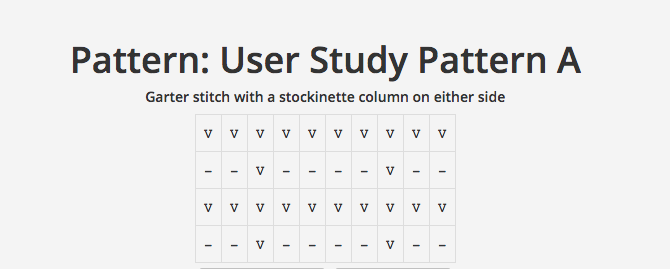
\includegraphics[width=5in]{nonresponsive_pattern_A}

\clearpage

\subsubsection{PurlPal}

\qquad \textbf{Description of Interface - Script} \label{script}

\medskip

\fbox{%
  \parbox{\textwidth}{%

  \medskip
    This is PurlPal!

    \medskip

    PurlPal will track your knitting as you move through the pattern using this sensor.
    The sensor isn't perfect, so you can also navigate through the pattern by using voice commands like ``move forward'' to go to the next stitch or ``next row'' to move to the beginning of the next row.
    You can also use these buttons or double click on any stitch to jump anywhere in the pattern.

    \medskip

    By default, PurlPal shows a chart of how the pattern looks from the right side.
    You are also welcome to look at the chart from the wrong side, or toggle between the right side and wrong side as you knit, by using these buttons.

    \medskip

    If you want to turn off motion detection or voice recognition, or you want to see available voice commands, you can find those in the settings menu here.

    \medskip

    Please get into position to start knitting so I can calibrate the sensor - but don't actually start yet.
    \\ ** calibrate sensor *
    \\ Okay, you can begin now. \medskip

  }%
}

\medskip

\textbf{Interface Example} \label{responsive}

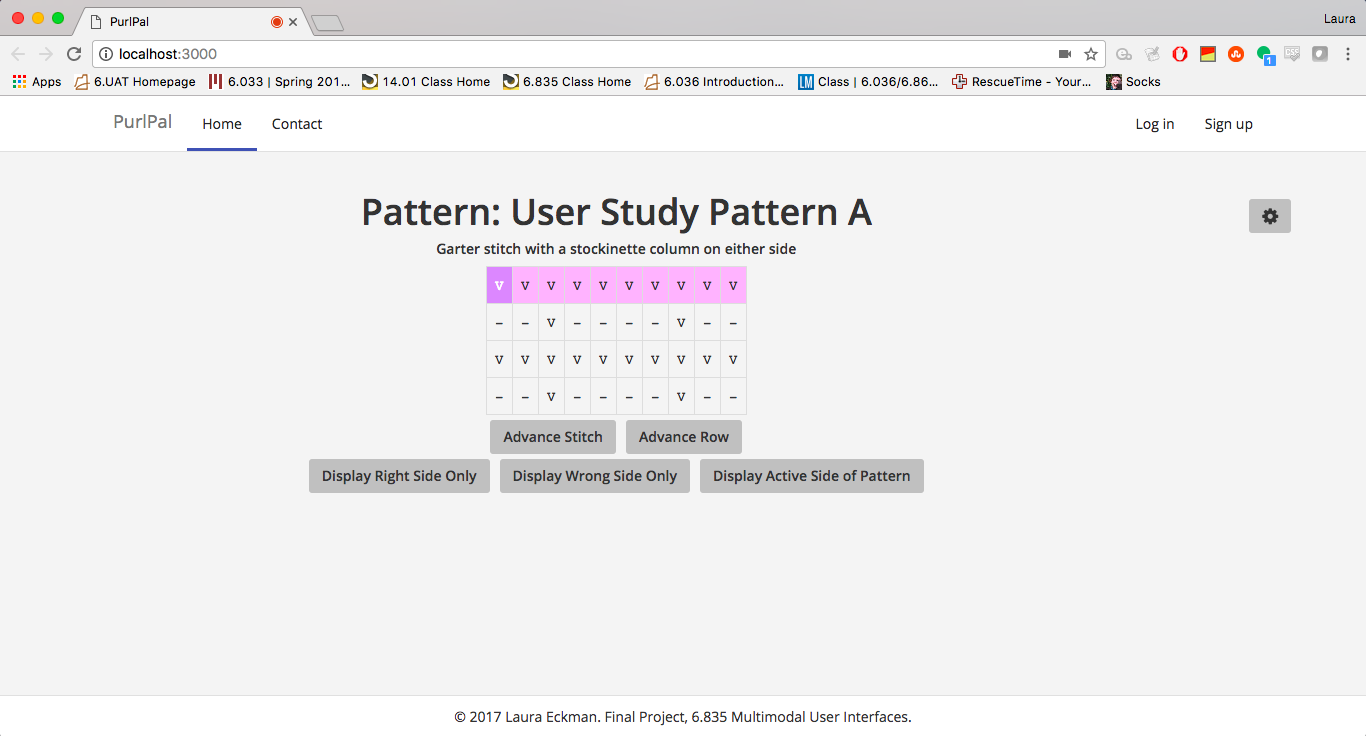
\includegraphics[width=6in]{responsive_pattern_A}

\subsection{PurlPal Questionnaire} \label{questionnaire}

\fbox{%
  \parbox{\textwidth}{%
    %\begin{center}
    \begin{enumerate}
      \item I found PurlPal easy to use. \\ \\
      Very True \qquad Mostly True \qquad Slightly True \qquad Slightly False \qquad Mostly False \qquad Very False
      \item I preferred navigating with speech rather than my mouse. \\ \\
      Very True \qquad Mostly True \qquad Slightly True \qquad Slightly False \qquad Mostly False \qquad Very False
      \item I preferred navigating with speech rather than motion detection. \\ \\
      Very True \qquad Mostly True \qquad Slightly True \qquad Slightly False \qquad Mostly False \qquad Very False
      \item I preferred navigating with motion detection rather than my mouse. \\ \\
      Very True \qquad Mostly True \qquad Slightly True \qquad Slightly False \qquad Mostly False \qquad Very False
      \item I would use a system like PurlPal for complex patterns only. \\ \\
      Very True \qquad Mostly True \qquad Slightly True \qquad Slightly False \qquad Mostly False \qquad Very False
      \item I would use a system like PurlPal for simple patterns only. \\ \\
      Very True \qquad Mostly True \qquad Slightly True \qquad Slightly False \qquad Mostly False \qquad Very False
      \item I prefer the row counting feature over tracking my place within the row. \\ \\
      Very True \qquad Mostly True \qquad Slightly True \qquad Slightly False \qquad Mostly False \qquad Very False
      \item I preferred knitting with PurlPal more than with the non-responsive pattern. \\ \\
      Very True \qquad Mostly True \qquad Slightly True \qquad Slightly False \qquad Mostly False \qquad Very False
      \\ \\ \\
      What features would you like to see added to PurlPal?
      \\ \\ \\ \\
      What, if any, features of PurlPal did you find unnecessary?
      \\ \\ \\ \\
      General Feedback:
      \\ \\ \\ \\
    \end{enumerate}
    %\end{center}
  }%
}

\end{document}
